O projeto de dados tem como objetivo retratar como serão persistidos os dados do sistema de forma a garantir integridade, consistência e eficiência no armazenamento das informações. Nesta etapa serão desenvolvidas as modelagens conceitual e lógica para representação do design da camada de persistência.

\subsection{Diagrama Conceitual}

De acordo com \citeonline{elmasri} o Diagrama Entidade-Relacionamento Estendido (DEER) trata-se de uma estrutura derivada de um modelo aprimorado da modelagem Entidade-Relacionamento. Tal modelo permite representar as conexões entre entidades de um sistema e os atributos dessas entidades, além de outras especificações destinadas ao banco de dados da aplicação. 

Nesta versão estendida, são incorporadas teorias de relacionamentos de classe e subclasse, em conjunto com herança de tipo, conceitos que possibilitam a representação de especializações e generalizações no diagrama \cite{elmasri}. O Diagrama Entidade-Relacionamento Estendido desenvolvido para este projeto está apresentado na Figura~\ref{der}. A notação adota tem como base os estudos de \citeonline{elmasri} com adaptações necessárias realizadas em função das limitações de correspondência de notação da ferramenta brModelo.

\begin{figure}[H]
    \centering
    \caption{Diagrama Entidade-Relacionamento do Projeto.}
    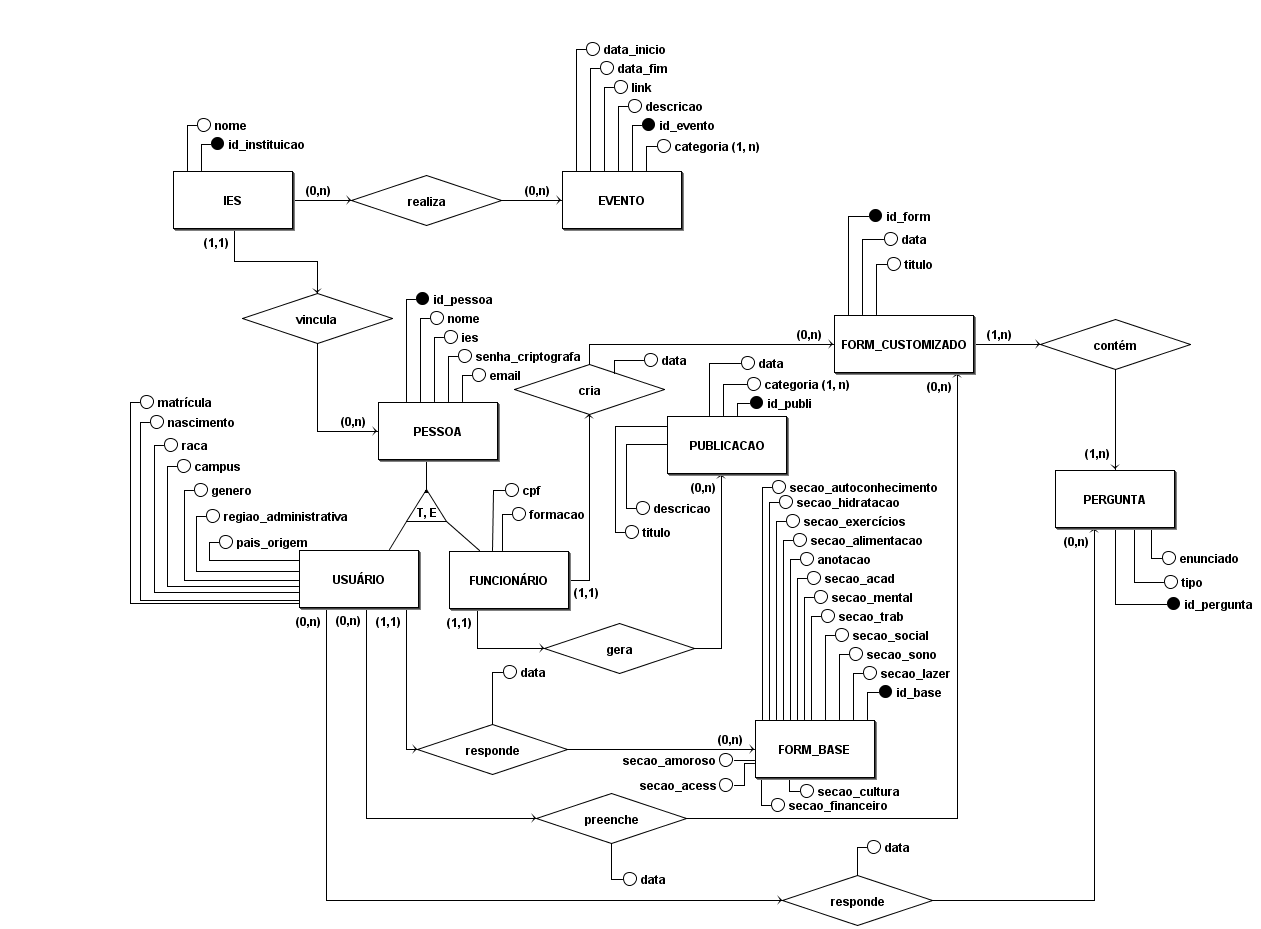
\includegraphics[width=0.65\textheight]{figuras/Conceitual.png}
    \par
    Fonte: autoria própria considerando as limitações do brModelo e com base em \citeonline{elmasri}.
    \par
    \label{der}
\end{figure}

\subsection{Diagrama Lógico}

O modelo lógico, de acordo com \citeonline{heuser2009projeto} "é uma descrição de um banco de dados no nível de abstração visto pelo usuário do Sistema Gerenciador de Banco de Dados (SGBD)". Assim, este modelo varia conforme o SGBD adotado. Neste trabalho, os tipos de dados foram definidos de forma condizente aos tipos disponíveis no PostgreSQL, tecnologia escolhida para este projeto.

Em outras palavras, neste diagrama é possível identificar de modo gráfico as tabelas que existirão no banco de dados além de suas respectivas colunas. O diagrama lógico de dados baseado no DEER mostrado anteriormente pode ser visto na Figura~\ref{ddl}.

\begin{figure}[H]
    \centering
    \caption{Diagrama Lógico do Projeto.}
    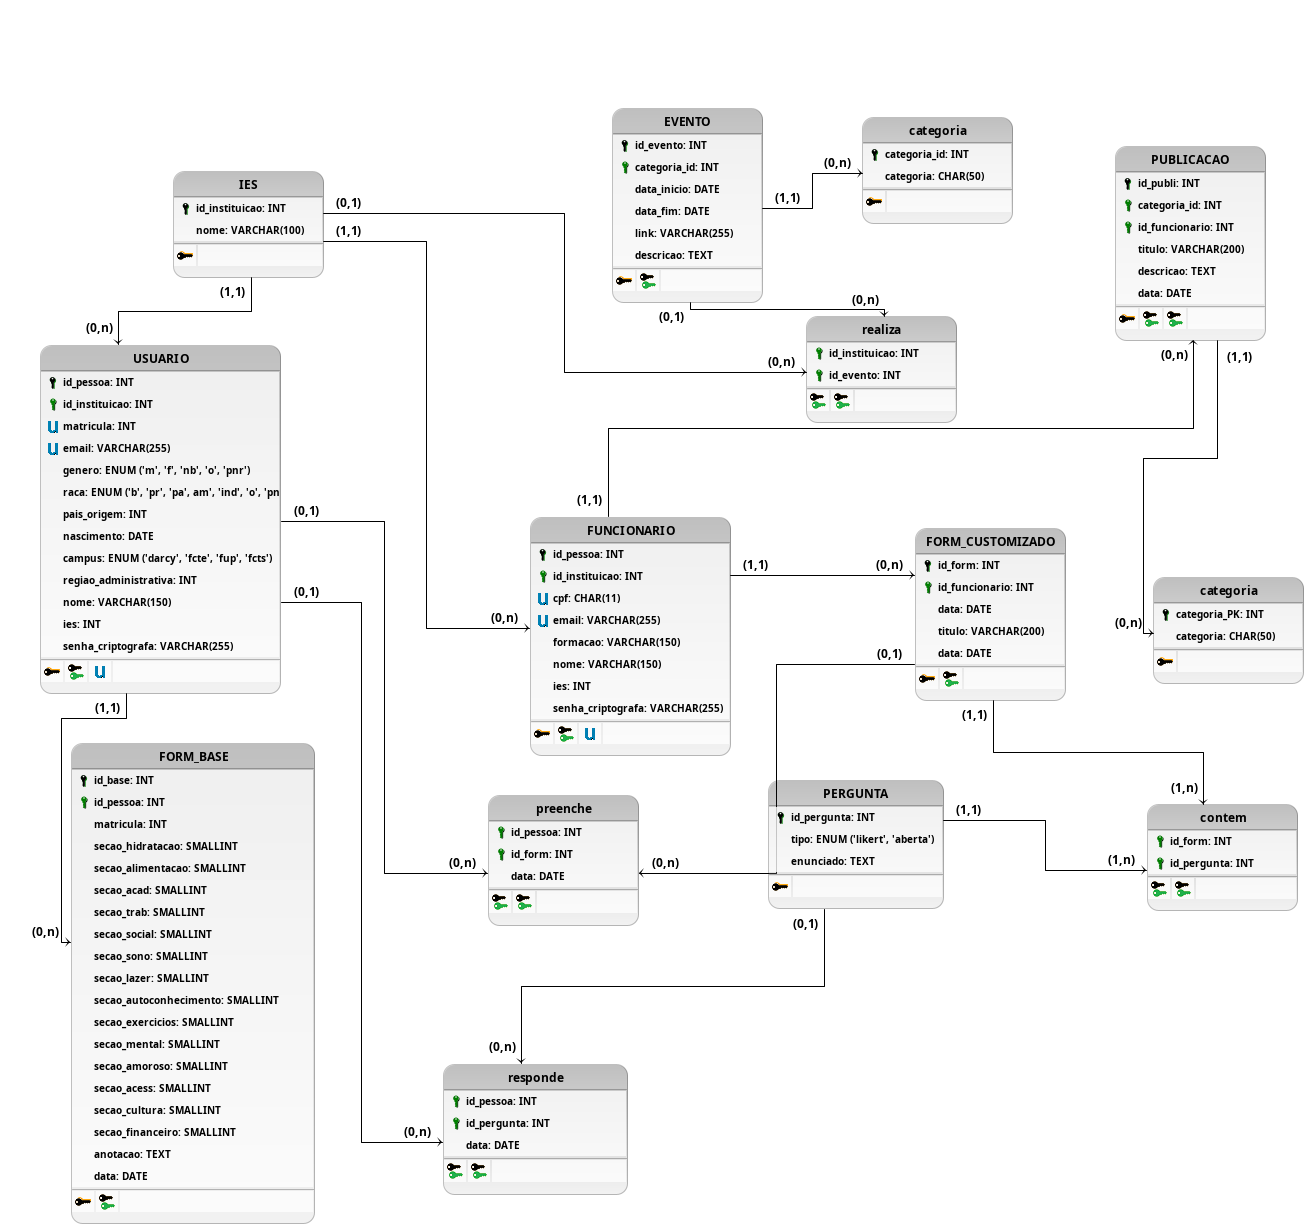
\includegraphics[width=0.65\textheight]{figuras/Lógico_1_atual.png}
    \par
    Fonte: autoria própria com auxílio da ferramenta de modelagem brModelo.
    \par
    \label{ddl}
\end{figure}

%\subsection{Dicionário de Dados}
%TODO ESCREVER AQUI
